\chapter*{Lecture 3}
\begin{recall}{}{}
\begin{itemize}
\item Order of an ODE
\item Linearity
\item Homogeneous
\item Constant/non-constant coefficient
\end{itemize}
\end{recall}

\subsection{Multiplicity of Solutions}
Let's take a step back. When you studied the concept of integration in calculus, you learned about constants of integration, for example:
\begin{equation*}
y'=e^x,
\end{equation*}
the solution is $y=e^x+c$ (where $c$ can take any numerical value). Similarly, if we have:
\begin{equation*}
y''=e^x,
\end{equation*}
the solution, by integrating twice, is: $y=e^x+c_1x+c_2$. Finally if we have:
\begin{equation*}
y'''=e^x,
\end{equation*}
The solution is $y=e^x+c_1x^2+c_2x+c_3$\\
From this simple example, we see that:
\begin{itemize}
\item if a differential equation has a solution, it has infinitely many solutions (coefficients $c$ can have infinitely many values).
\item if the differential equation is of  $n$-order, its solution contains $n$ arbitrary constants.
\end{itemize}

\subsection{General vs Particular solution}
\begin{itemize}
\item  A \textbf{general solution} to a differential equation is a solution from which every particular solution may be obtained by an appropriate choice of values for arbitrary constants.
\item A \textbf{particular solution} to a differential equation is a function that satisfies the differential equation, but contains no arbitrary constants.
\end{itemize}





\subsection{Definition of an IVP}
\textbf{Initial value problem (IVP)}:  a problem that can be described by an ODE and a set of initial conditions (ICs) which are the known values of the function and its derivative (if necessary) at the independent variable equal to zero (or initial state).

\begin{testv}{Number of ICs}{}
The number of initial conditions required to fully define a solution equals the order of the ODE
\end{testv}

\begin{center}
\noindent\rule{4cm}{0.4pt}
\end{center}

\subsection{Example: IVP}
\begin{exmp}
The function $y(x)=c_1 e^{-x}+c_2e^{2x}$ is a solution to:
\begin{equation}
\frac{d^2 y}{dx^2}-\frac{dy}{dx}-2y=0
\end{equation}
for any constant $c_1$ and $c_2$ (homework: verify). Determine the coefficients so that the initial conditions:  $y(0)=2$ and $\frac{dy(0)}{dx}=-3$ are satisfied.\\
\textbf{Solution:}  We compute: $\frac{d y}{dx}=-c_1e^{-x}+2c_2e^{2x}$. By substituting the ICs into our system of equations, we get:
\begin{eqnarray}
y(0)=c_1e^0+c_2e^0=2\\
\frac{dy(0)}{dx}=-c_1e^0+2c_2e^0=-3
\end{eqnarray}
Or by simplification, we get the following system of equations:
\begin{eqnarray}
c_1+c_2=2\\
-c_1+2c_2=-3
\end{eqnarray}
Through a bit of manipulations, we find: $c_1=7/3$ and $c_2=-1/3$. The solution to our IVP is then: $y(x)=7/3 e^{-x}-1/3e^{2x}$. $\bLozenge$
\end{exmp}
\begin{center}
\noindent\rule{4cm}{0.4pt}
\end{center}


\section{Direction Fields (optional)}
Let's consider a first-order differential equation in the form:
\begin{equation}
\frac{dy}{dx}=f(x,y)
\end{equation}
 If we can compute the function $f$, we know the slope at every point. This allows us to visualize the solution of the ODE.

\begin{exmp}
Let's take for instance the following ODE:
\begin{equation}
\frac{dy}{dx}=4-3x -y \qquad (\text{over }\infty<x<\infty)
\end{equation}
\begin{figure}
\centering
\includegraphics[width=0.48\textwidth]{figs/DirectionalField.pdf} 
\includegraphics[width=0.49\textwidth]{figs/DirectionField.pdf} 
\caption{Example of direction field \label{exDirField}}
\end{figure}
We can find a particular solution by stating that the solution passes by the point e.g. (2,-1). (see figure \ref{exDirField})
\end{exmp}

\subsection{Method of isoclines}
To simplify the drawing of the direction field, we can draw the \textbf{isoclines} of the equation. 
Suppose we have:
\begin{equation}
\frac{dy}{dx} = F(x,y)= x+y
\end{equation}
If find the isocline at which the slope is constant, say 3, we can write: $y=-x + 3$. Similarly, we can do this for all slopes in the curve.


%
%
%\section{Physical implications of first-order ODE}
%\begin{enumerate}
%\item The velocity of an object:
%\begin{equation}
%\vec{u}=\frac{d\vec{x}}{dt}
%\end{equation}
%The vector $\vec{u}$ tells us information on the direction of the movement.
%\item Mass diffusion: A container is divided into two chambers at $t=t_0$. We inject $H_2$ into the left chamber until the concentration reaches $C_L=10$ mole/cc. The right chamber has no $H_2$.
%
%We then remove the plate at moment $t=t_1$, we build up a gradient in the concentration of hydrogen such that:
%\begin{equation}
%\frac{d C}{dx}=\frac{C_L-C_R}{dx}
%\end{equation}
%The diffusion of hydrogen is driven by the gradient.\\
%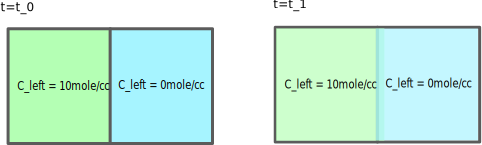
\includegraphics[width=0.8\textwidth]{figs/concentration.pdf} 
%\end{enumerate}
%
%
%
%\section{Examples}
%\begin{exmp}{Streamlines in fluid mechanics}
%
%\end{exmp}
%

\chapter{First-order Differential Equations}
In this chapter, we study analytical solution methods  of  \textbf{first-order  ODEs}.\\
\begin{itemize}
\item Unfortunately only some types of ODEs have solutions! (we will learn these types)
\item There is no connection between the appearance of a differential equation and the ease of finding a solution. $\frac{dy}{dx}=x^2+y$ and $\frac{dy}{dx}=x^2+y^2$ look similar, yet the first has a solution, the second does not.
\end{itemize}

\section{Overview of Solution approaches}
\begin{itemize}
\item Direct integration (separable equation)
\item Substitution and transformation
\item Exact equations
\item Integrating factors
\item First-order linear ODE formula
\end{itemize}




\section{Direct integration}
A solution can be found using direct integration if we are able to \textbf{separate the differential equation}.\\

Definition: An equation is \textbf{separable} if the RHS of a first-order equation of the form:
\begin{equation}
\frac{dy}{dx}=f(x,y)
\end{equation}
can be expressed as a function $g(x)$ and $p(y)$. In other words, if we can write the equation in the form:
\begin{equation}
\frac{dy}{dx}=g(x)p(y)
\label{sepEq}
\end{equation}

\begin{center}
\noindent\rule{4cm}{0.4pt}
\end{center}

\begin{exmp}{} Are the following equations separable?
\begin{equation*}
\frac{dy}{dx}=-\frac{x}{y^2}= \left(-x\right)\left(\frac{1}{y^2}\right) \qquad \text{separable}
\end{equation*}
\begin{equation*}
\frac{dy}{dx}=1+xy \qquad \qquad \text{not separable}
\end{equation*}
\end{exmp}
\begin{center}
\noindent\rule{4cm}{0.4pt}
\end{center}


\subsection*{Solution of a separable equation}
To solve the equation \eqref{sepEq}
\begin{enumerate}

\item[Step 1] separate the dependent and independent variable on either side of the equation such that:
\begin{equation}
\frac{dy}{p(y)}=g(x){dx}
\end{equation}
\item[Step 2] integrate both sides:
\begin{equation}
\int{\frac{1}{p(y)}dy}=\int{g(x){dx}}
\end{equation}
The equation sometimes gives an implicit solution to the ODE.
\item[Step 3] Determine the integration constant (apply ICs).
\end{enumerate}

\begin{center}
\noindent\rule{4cm}{0.4pt}
\end{center}

\begin{exmp}{} Solve:
\begin{equation}
\frac{dy}{dx}=\frac{4x}{1+2e^y}
\end{equation}
with the initial condition $y(0)=1$.\\
(1st order, non-linear, SEPARABLE, ODE)\\
\textbf{Solution:}
\begin{enumerate}
\item[Step 1] Separate the ODE:
\begin{equation}
\left(1+2e^y\right){dy}={4x}{dx}
\end{equation}
\item[Step 2] Integrate both sides:
\begin{equation}
\int{\left(1+2e^y\right)}{dy}=\int{{4x}}{dx}
\end{equation}
we obtain:
\begin{equation}
y+2e^y=2x^2 + C
\end{equation}
This is the \textbf{general solution}.\\
DO not forget about integrative constants!
\item[Step 3] Determine the value of the integration constant $C$ by applying the initial condition. \\
At $x=0$, we have $y=1$, therefore, we can replace in our general solution to obtain:
\begin{equation}
(1)+2e^{(1)}=2(0)^2 + C
\end{equation}
We find: $C=1+2e$\\
The final (particular) solution to the ODE is:
\begin{equation}
\boxed{y+2e^y=2x^2 + 1+2e}
\end{equation}
\end{enumerate}
\end{exmp}
\begin{center}
\noindent\rule{4cm}{0.4pt}
\end{center}

\updateinfo[September 12, 2018]
